\section{Results}

In this section we explore and discuss the results of our experiments with the machine learning, deep learning, and transformer models for Pashto poetry classification. We present the results of our experiments in the following subsections. 

\subsection{Machine Learning Models}

This subsection presents the results of our experiments with the machine learning models. We used the following machine learning models for our experiments: Random Forest, Support Vector Machine, Logistic Regression, and XGBoost. The dataset was divided into 21844 samples for training, and 5465 samples for testing. The models were trained on an 8 Core, 4.90 GHz Intel Core i7-12700 CPU with 16GB RAM. 

\subsubsection{Random Forest}
Using 100 estimators, and a max depth of None, the Random Forest model achieved an accuracy of 51.93\%, and an F1 score of 0.50. The confusion matrix for the Random Forest model is shown below:
\begin{figure}[H]
    \centering
    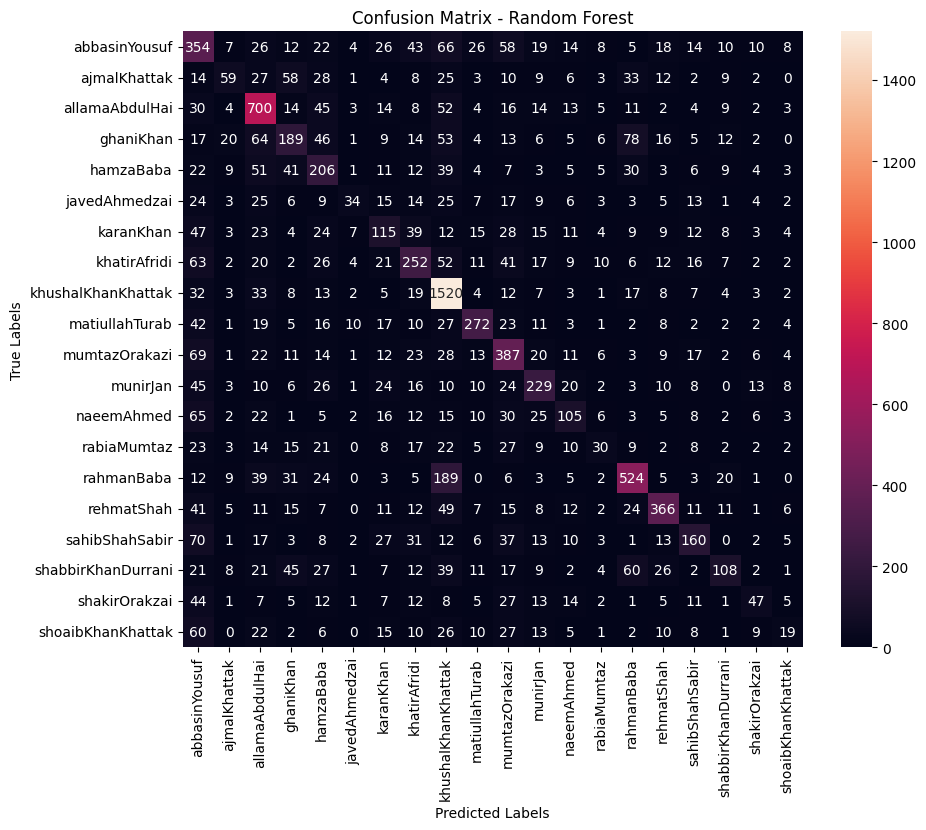
\includegraphics[width=0.4\textwidth]{rf_confmat.png}
\end{figure}

\subsubsection{Support Vector Machine}
With a C value of 1.0, an `rbf' kernel, and a gamma value of `scale', the Support Vector Machine model achieved an accuracy of 61.92\%, and an F1 score of 0.60. The confusion matrix for the Support Vector Machine model is shown below:
\begin{figure}[H]
    \centering
    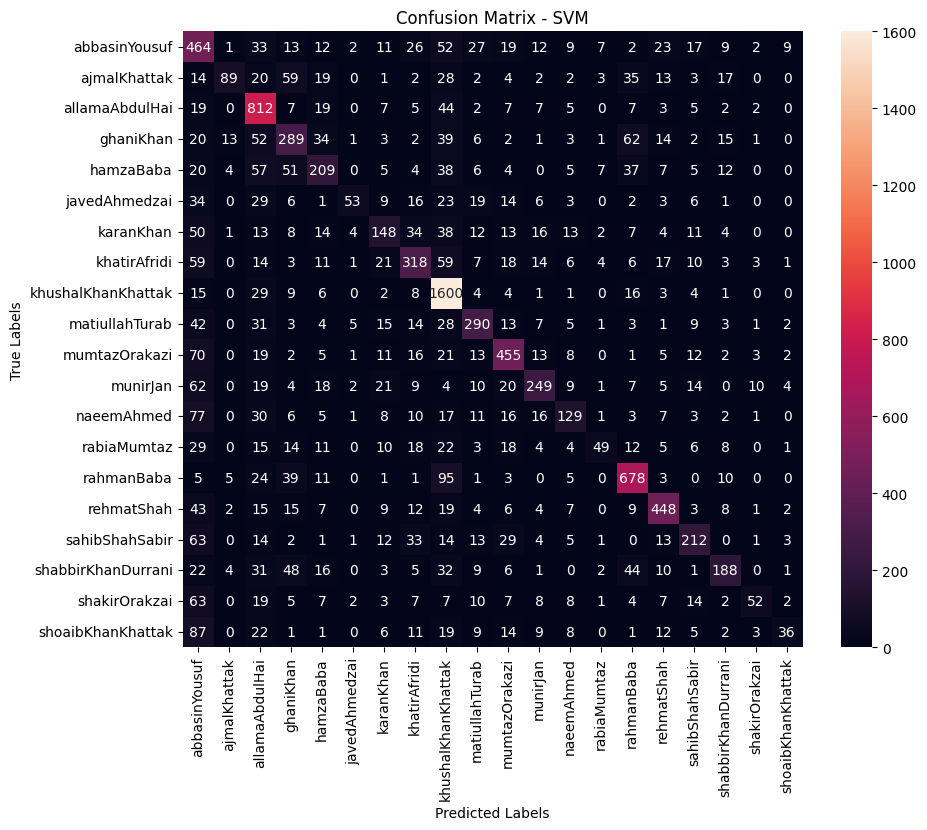
\includegraphics[width=0.4\textwidth]{svm_confmat.png}
\end{figure}

\subsubsection{Logistic Regression}
For the Logistic Regression model, our best hyperparameters turned out to be a C value of 10, max iterations of 1000, and a `newton-cg' solver. This gave an accuracy of 62.88\%, and an F1 score of 0.62. The confusion matrix for the Logistic Regression model is shown below:
\begin{figure}[H]
    \centering
    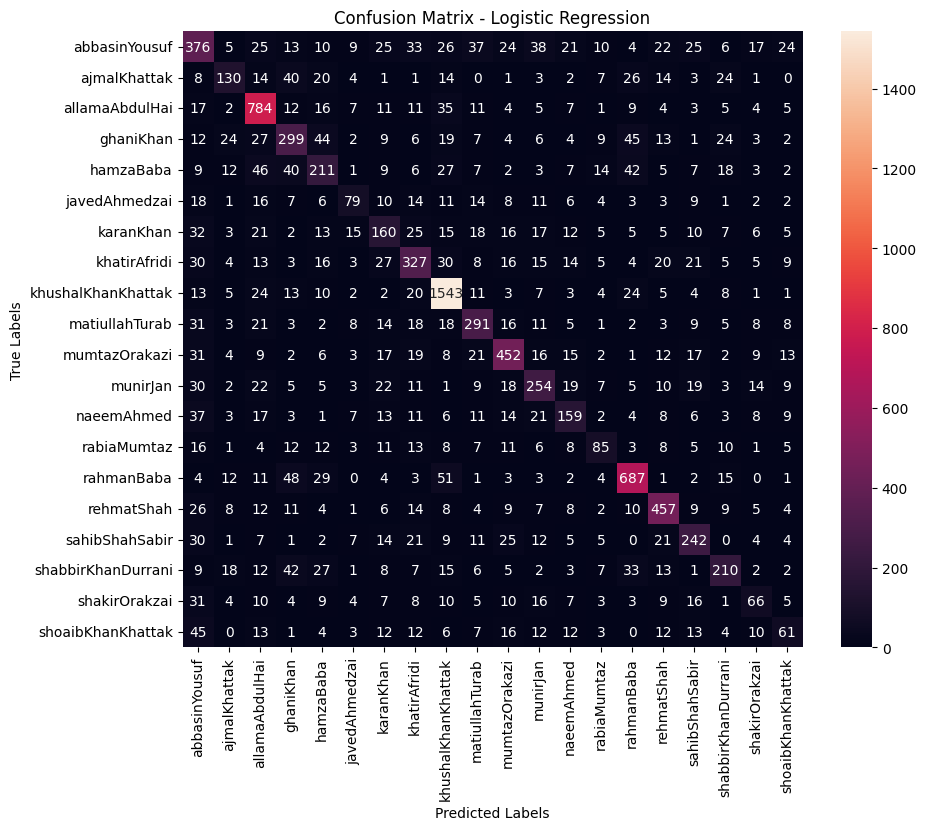
\includegraphics[width=0.4\textwidth]{logreg_confmat.png}
\end{figure}

\subsubsection{XGBoost}
Our best hyperparameters for XGBoost were 100 estimators, a learning rate of 0.1, max depth of 3, gamma value of 0.1, and a log-loss evaluation metric. This gave us an accuracy of 41.67\% and an F1 Score of 0.38. The confusion matrix for the XGBoost model is shown below:
\begin{figure}[H]
    \centering
    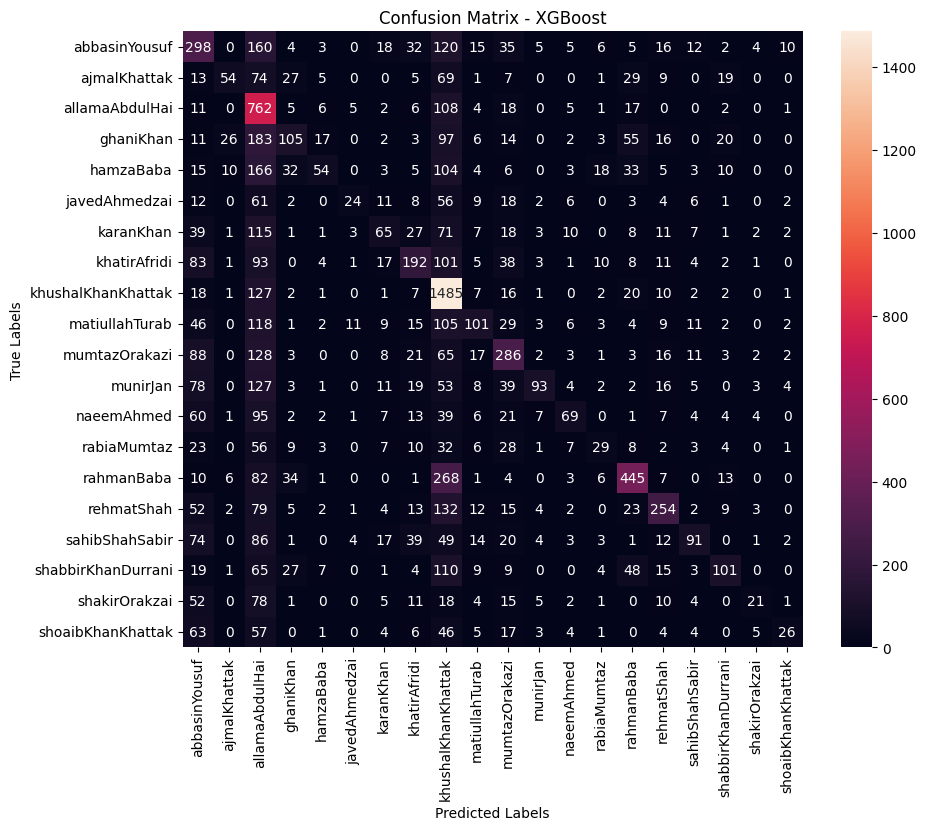
\includegraphics[width=0.4\textwidth]{xgboost_confmat.png}
\end{figure}

\subsection{Deep Learning Models}

This subsection presents the results of our experiments with the deep learning models. We used the following deep learning models for our experiments: LSTM and Bi-LSTM. The dataset was divided into 19111 samples for training, 2727 samples for validation, and 5471 samples for testing. They were trained on 2 Tesla T4 GPUs available on Kaggle, with Kaggle's 29GB RAM. 

\subsubsection{LSTM}
We experimented with various layers, and hyperparameters for LSTM including Bi-LSTM layers as well. Interestingly, the model was performing better on the TF-IDF features rather than embeddings, so even though our initial pipeline mentioned that the model would be trained on embeddings, we decided to train the LSTM model on the TF-IDF features rather than the embeddings as they were giving comparatively better results. The models were trained on 20 Epochs, with early stopping enabled. We experimented with a simple LSTM model with 2 LSTM layers of 128 and 64 units, respectively. We also added 2 dropout layers, and a dense layer with 64 units. The model was overfitting the training data, hence we continued with different parameters including compiling with an Adam Optimizer with a learning rate of 0.001, and a sparse categorical cross entropy loss, but that as well overfitted with a poor accuracy on the validation and test sets. Our final model was a Bi-LSTM model with a Dense layer with a softmax activation function, compiled using the Adam Optimizer with a learning rate of 0.0001, sparse categorical cross entropy loss, and an early stopping layer. The model achieved an accuracy of 59.63\% on the test set. The plots and confusion matrix for the Bi-LSTM Model are shown as follows:

\begin{figure}[H]
    \centering
    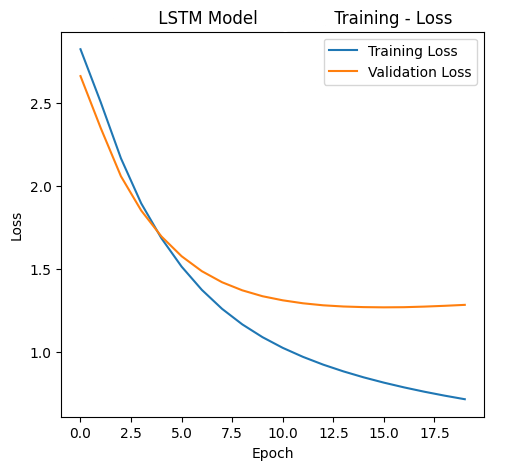
\includegraphics[width=0.4\textwidth]{dl_lstm_trainloss.png}
    \caption{Training Loss for LSTM Model}
    \label{fig:dl_lstm_trainloss}
\end{figure}

\begin{figure}[H]
    \centering
    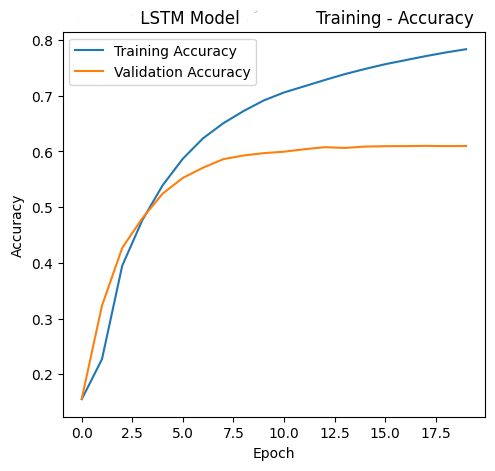
\includegraphics[width=0.4\textwidth]{dl_lstm_trainaccuracy.png}
    \caption{Training Accuracy for LSTM Model}
    \label{fig:dl_lstm_trainaccuracy}
\end{figure}

\begin{figure}[H]
    \centering
    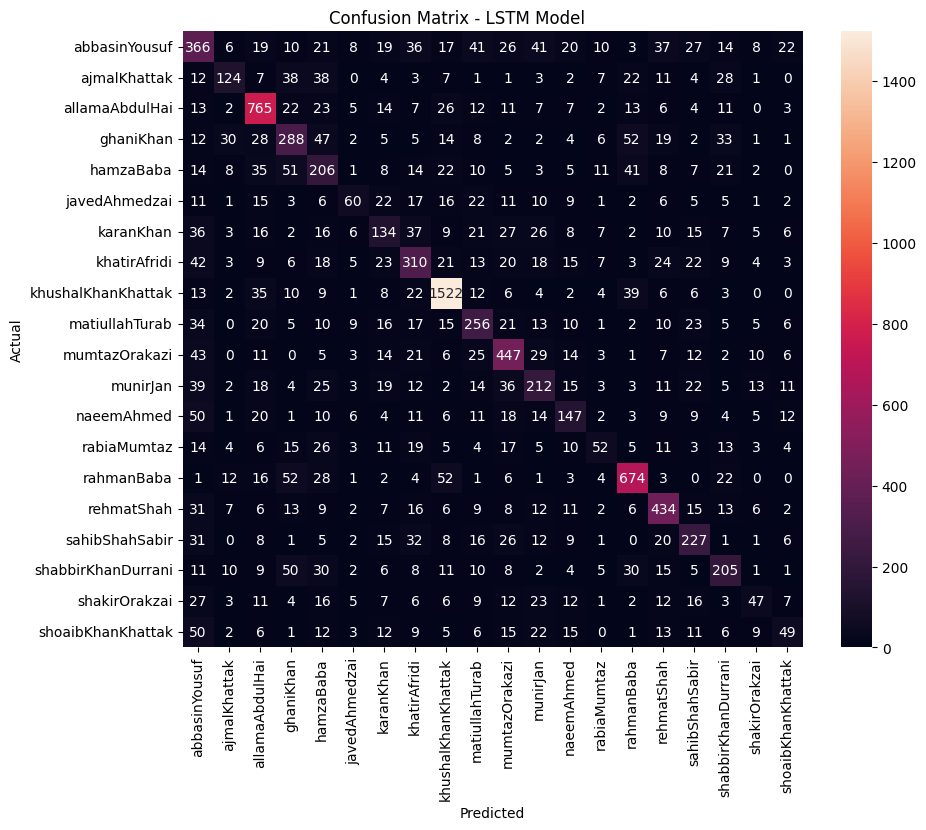
\includegraphics[width=0.4\textwidth]{dl_lstm_confmat.png}
    \caption{Confusion Matrix for LSTM Model}
    \label{fig:dl_lstm_confmat}
\end{figure}

\subsection{Transformer Models}

This subsection presents the results of our experiments with the transformer models. We used the following transformer models for our experiments: roBERTa, DistilBERT, and Meta Llama-3.2-1b. The embeddings generated were trained on 2 Tesla T4 GPUs available on Kaggle, with Kaggle's 29GB RAM.

\subsubsection{DistilBERT}
The model was trained on 100 epochs with early stopping, a batch size of 32, with an Adam optimizer with learning rate of 0.001, and cross entropy loss function. The model was only able to achieve an accuracy of 45.39\%. The plots and confusion matrix for the DistilBERT Model are shown as follows:

\begin{figure}[H]
    \centering
    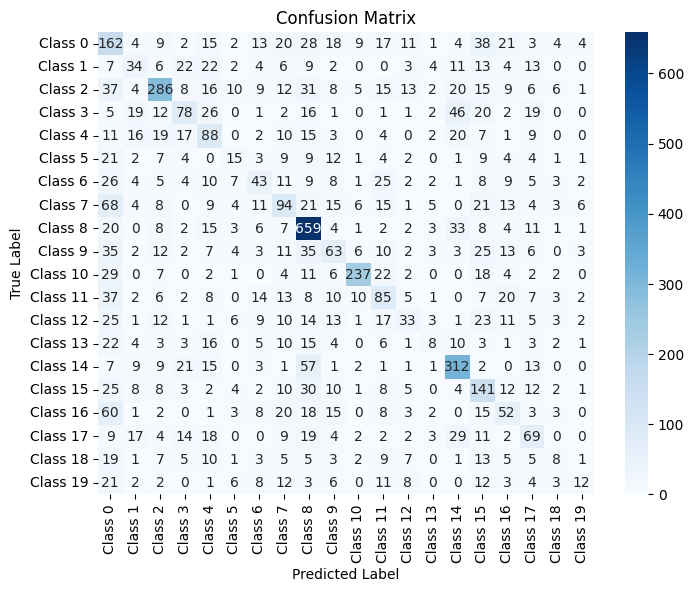
\includegraphics[width=0.4\textwidth]{distilbert_confmat.png}
    \caption{Confusion Matrix for DistilBERT Model}
    \label{fig:distilbert_confmat}
\end{figure}

\begin{figure}[H]
    \centering
    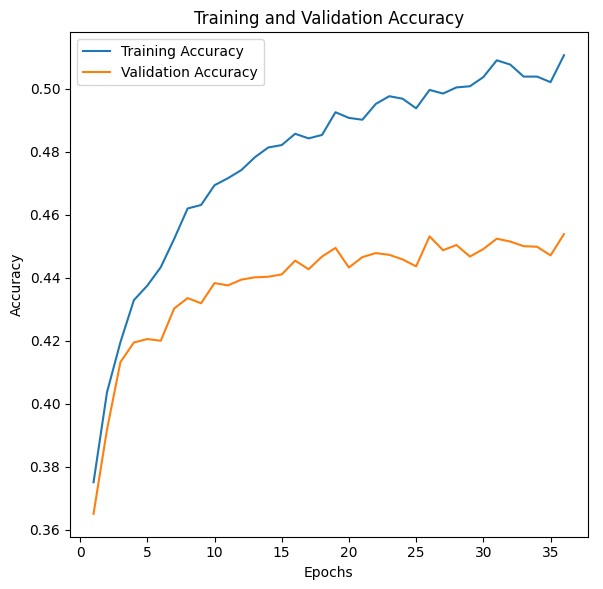
\includegraphics[width=0.4\textwidth]{distilbert_trainaccuracy.png}
    \caption{Training Accuracy for DistilBERT Model}
    \label{fig:distilbert_trainaccuracy}
\end{figure}

\subsubsection{Meta Llama-3.2-1b}

The Meta Llama 3.2 1b parameter model was trained on 20 epochs, with a batch size of 8, learning rate of 0.001, the Adam optimizer, and cross entropy loss function, with an early stopping. The model only achieved an accuracy of 48.88\%. The plots and confusion matrix for the Meta Llama-3.2-1b Model are shown as follows:

\begin{figure}[H]
    \centering
    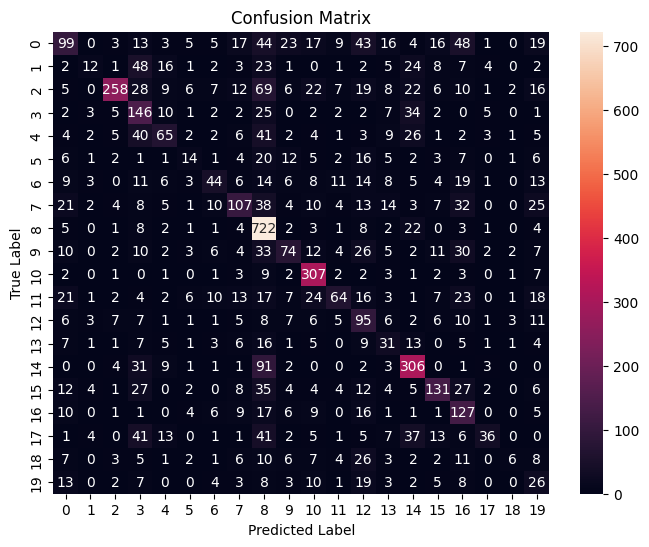
\includegraphics[width=0.4\textwidth]{llama_confmat.png}
    \caption{Confusion Matrix for Meta Llama-3.2-1b Model}
    \label{fig:llama_confmat}
\end{figure}

\begin{figure}[H]
    \centering
    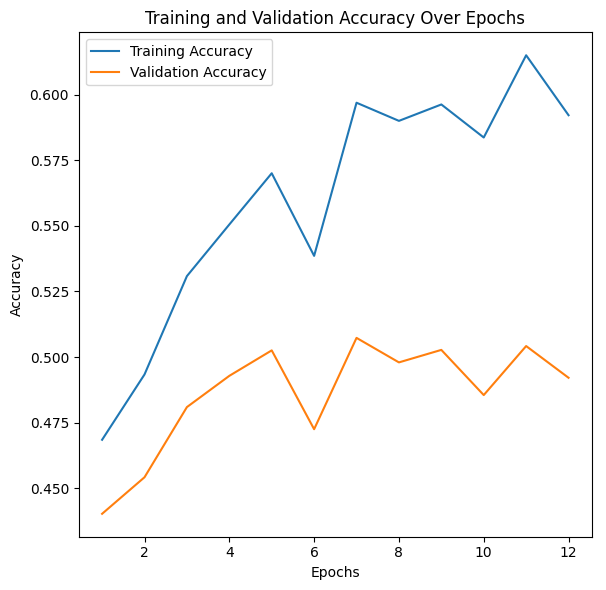
\includegraphics[width=0.4\textwidth]{llama_trainaccuracy.png}
    \caption{Training Accuracy for Meta Llama-3.2-1b Model}
    \label{fig:llama_trainaccuracy}
\end{figure}

% \begin{figure}[H]
%     \centering
%     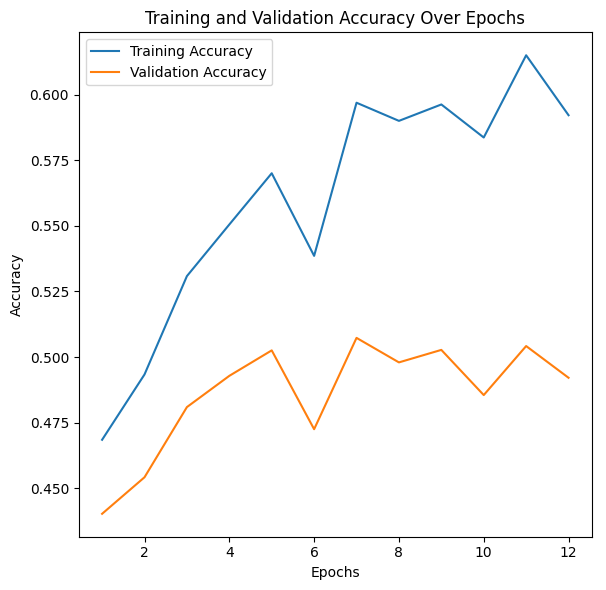
\includegraphics[width=0.4\textwidth]{llama_trainloss.png}
%     \caption{Training Loss for Meta Llama-3.2-1b Model}
%     \label{fig:llama_trainloss}
% \end{figure}

\subsubsection{Bert Based Multilingual Uncased}
As above, the model was trained on 100 epochs, with a batch size of 8, learning rate of 0.001, the Adam optimizer, and cross entropy loss function, with an early stopping. The model only achieved an accuracy of 49.25\%. The plots and confusion matrix for the Bert Based Multilingual Uncased Model are shown as follows:

\begin{figure}[H]
    \centering
    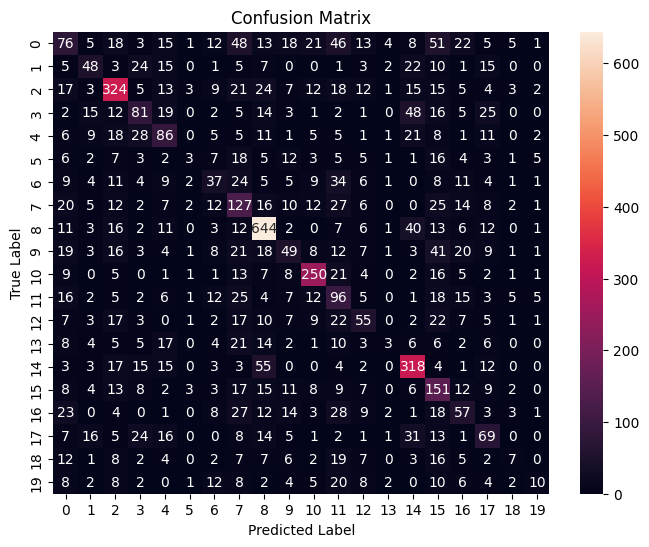
\includegraphics[width=0.4\textwidth]{bbmu_confmat.png}
    \caption{Confusion Matrix for Bert Based Multilingual Uncased Model}
    \label{fig:bbmu_confmat}
\end{figure}

\begin{figure}[H]
    \centering
    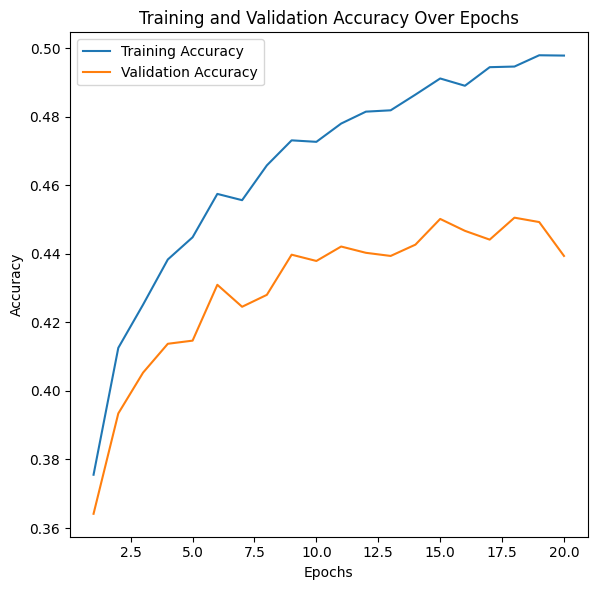
\includegraphics[width=0.4\textwidth]{bbmu_trainaccuracy.png}
    \caption{Training Accuracy for Bert Based Multilingual Uncased Model}
    \label{fig:bbmu_trainaccuracy}
\end{figure}

% \begin{figure}[H]
%     \centering
%     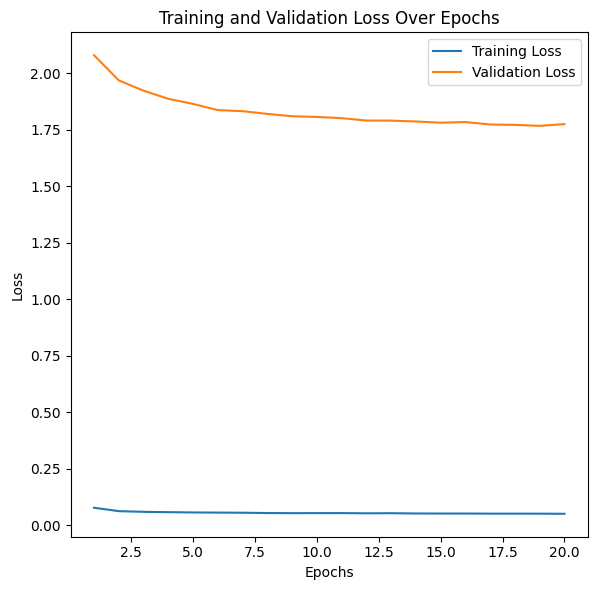
\includegraphics[width=0.4\textwidth]{bbmu_trainloss.png}
%     \caption{Training Loss for Bert Based Multilingual Uncased Model}
%     \label{fig:bbmu_trainloss}
% \end{figure}

\subsubsection{Mt5 Multilingual XLSum}
We experimented with various hyperparameters for this model as well. The best performance we got was on 100 epochs with early stopping, a batch size of 8, a Stochastic Gradient Descent optimizer with a learning rate of 0.01 and momentum of 0.9, and a cross entropy loss function. The model only achieved an accuracy of 44.40\%. The plots and confusion matrix for the Mt5 Multilingual XLSum Model are shown as follows:

\begin{figure}[H]
    \centering
    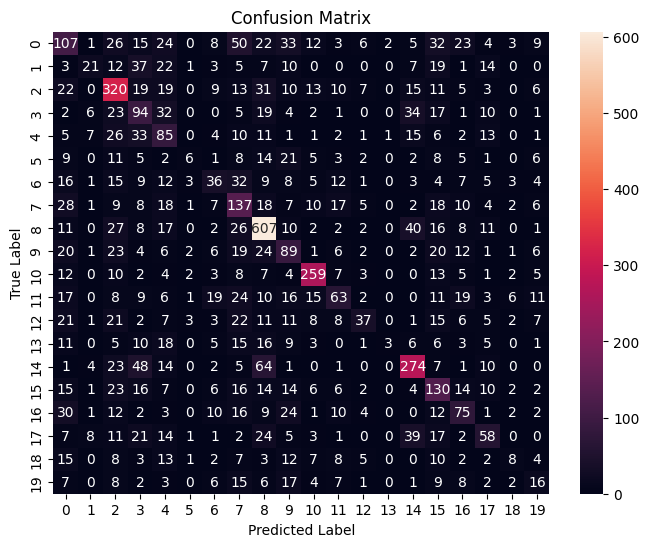
\includegraphics[width=0.4\textwidth]{mt5_confmat.png}
    \caption{Confusion Matrix for Mt5 Multilingual XLSum Model}
    \label{fig:mt5_confmat}
\end{figure}

\begin{figure}[H]
    \centering
    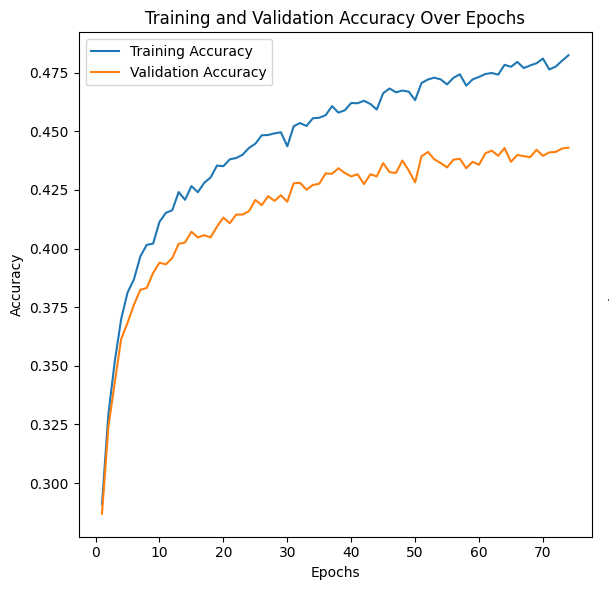
\includegraphics[width=0.4\textwidth]{mt5_trainaccuracy.png}
    \caption{Training Accuracy for Mt5 Multilingual XLSum Model}
    \label{fig:mt5_trainaccuracy}
\end{figure}

% \begin{figure}[H]
%     \centering
%     \includegraphics[width=0.4\textwidth]{mt5_trainloss.png}
%     \caption{Training Loss for Mt5 Multilingual XLSum Model}
%     \label{fig:mt5_trainloss}
% \end{figure}

\subsubsection{MT0-Base}
The model was trained on 200 epochs with early stopping, a batch size of 8, the Stochastic Gradient Descent optimizer with a learning rate of 0.01 and a momentum of 0.9, and a cross entropy loss function. The model only achieved an accuracy of 50.24\%. The plots and confusion matrix for the MT0-Base Model are shown as follows:

\begin{figure}[H]
    \centering
    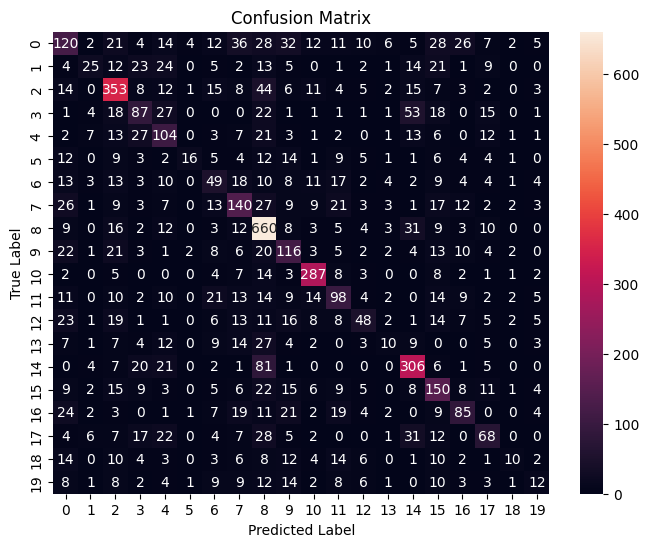
\includegraphics[width=0.4\textwidth]{mt0_confmat.png}
    \caption{Confusion Matrix for MT0-Base Model}
    \label{fig:mt0_confmat}
\end{figure}

\begin{figure}[H]
    \centering
    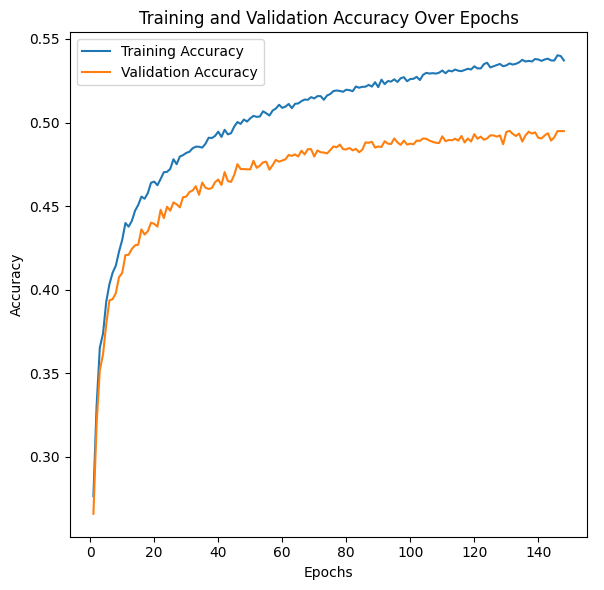
\includegraphics[width=0.4\textwidth]{mt0_trainaccuracy.png}
    \caption{Training Accuracy for MT0-Base Model}
    \label{fig:mt0_trainaccuracy}
\end{figure}

% \begin{figure}[H]
%     \centering
%     \includegraphics[width=0.4\textwidth]{mt0_trainloss.png}
%     \caption{Training Loss for MT0-Base Model}
%     \label{fig:mt0_trainloss}
% \end{figure}

\subsection{Summary of Results}

This subsection presents a summary of the results of our experiments with the machine learning, deep learning, and transformer models for Pashto poetry classification.

\begin{table}[ht]
    \centering
    \begin{tabular}{|l|l|c|}
        \hline
        \textbf{Type} & \textbf{Model} & \textbf{Accuracy} \\
        \hline
        ML model & Logistic Regression & 62.88\% \\
        ML model & Support Vector Machine & 61.92\% \\
        DL Based model & Bi-LSTM & 59.63\% \\
        ML model & Random Forest & 51.93\% \\
        DL Based model & MT0-Base & 50.24\% \\
        DL Based model & Bert Based Multilingual Uncased & 49.25\% \\
        DL Based model & Meta Llama-3.2-1b & 48.88\% \\
        DL Based model & DistilBERT & 45.39\% \\
        DL Based model & Mt5 Multilingual XLSum & 44.40\% \\
        ML model & XGBoost & 41.67\% \\
        \hline
    \end{tabular}
    \caption{Table of Results}
    \label{tab:results}
\end{table}




